\documentclass[12pt]{article}

% a template that a friend gave, it's worked well enough for me
% i have added some packages and stuff that have proved useful

\usepackage{fancyhdr}
\usepackage{tipa}
\usepackage{fontspec}
\usepackage{amsfonts}
\usepackage{enumitem}
\usepackage[margin=1in]{geometry}
\usepackage{graphicx}
\usepackage{float}
\usepackage{amsmath}
\usepackage{braket}
\usepackage{amssymb}
\usepackage{booktabs}
\usepackage{hyperref}
\usepackage{mathtools}
\usepackage{xcolor}
\usepackage{float}
\usepackage{algpseudocodex}
\usepackage{titlesec}
\usepackage{bbm}

\pagestyle{fancy}
\fancyhf{} % sets both header and footer to nothing
\lhead{Kevin Sheng}
\setmainfont{Comic Neue}
\renewcommand{\headrulewidth}{1pt}
\setlength{\headheight}{0.75in}
\setlength{\oddsidemargin}{0in}
\setlength{\evensidemargin}{0in}
\setlength{\voffset}{-.5in}
\setlength{\headsep}{10pt}
\setlength{\textwidth}{6.5in}
\setlength{\headwidth}{6.5in}
\setlength{\textheight}{8in}
\renewcommand{\headrulewidth}{0.5pt}
\renewcommand{\footrulewidth}{0.3pt}
\setlength{\textwidth}{6.5in}
\usepackage{setspace}
\usepackage{multicol}
\usepackage{float}
\setlength{\columnsep}{1cm}
\setlength\parindent{24pt}
\usepackage [english]{babel}
\usepackage [autostyle, english = american]{csquotes}
\MakeOuterQuote{"}

\setlength{\parskip}{6pt}
\setlength{\parindent}{0pt}

\titlespacing\section{0pt}{12pt plus 4pt minus 2pt}{0pt plus 2pt minus 2pt}
\titlespacing\subsection{0pt}{12pt plus 4pt minus 2pt}{0pt plus 2pt minus 2pt}
\titlespacing\subsubsection{0pt}{12pt plus 4pt minus 2pt}{0pt plus 2pt minus 2pt}

\hypersetup{colorlinks=true, urlcolor=blue}

\newcommand{\correction}[1]{\textcolor{red}{#1}}


\allowdisplaybreaks

% i get homework drops
% and i've deemed this assignment a waste of my time

\begin{document}
\section{Textbook}\label{sec:textbook}

\subsection*{8.5}\label{sec:8.5}

\begin{enumerate}
      \item[5] \[\begin{bmatrix}
                        0 & 9 & 0 & 1 & 1 \\
                        0 & 0 & 0 & 1 & 1 \\
                        0 & 0 & 0 & 1 & 1 \\
                        1 & 1 & 1 & 0 & 0 \\
                        1 & 1 & 1 & 0 & 0
                  \end{bmatrix}\]
      \item[15] The graph consists of two connected components.
            \begin{center}
                  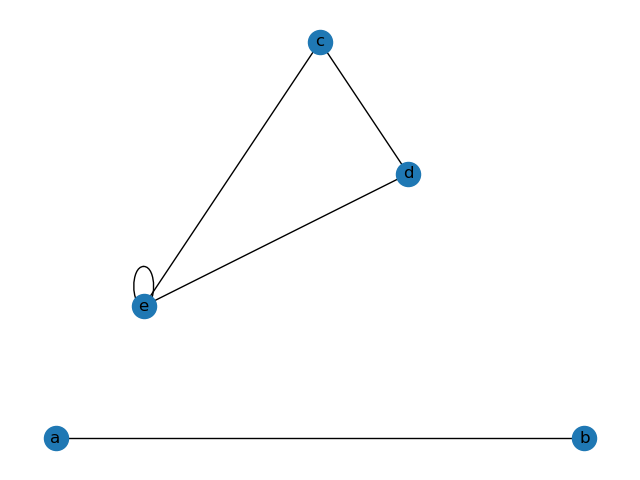
\includegraphics[width=10cm]{img/graph}
            \end{center}
\end{enumerate}

\subsection*{8.6}\label{sec:8.6}

\begin{enumerate}
      \item[2] It we assign the nodes $3$, $4$, $1$, $5$, and $2$ to the vertices
            $a$, $b$, $c$, $d$, and $e$ respectively,
            we can see that the two graphs have the same adjacency matrix.
      \item[11] The two graphs are not isomorphic, as the degress of their nodes are different.
      $G_1$ has degrees $[3, 4, 2, 4, 3]$, while $G_2$ has degrees $[4, 3, 3, 3, 3]$.
      \item[21] For our first graph, we can take $K_{3,3}$.
      \item[32]
\end{enumerate}

\subsection*{8.7}\label{sec:8.7}

\begin{enumerate}
      \item[2]
\end{enumerate}

\pagebreak

\section{Handout}\label{sec:handout}

\begin{itemize}
      \item[A1] SWOC that $T$ has no leaves.
            This would mean all vertices have to be of at least degree $2$,
            since a vertex with degree $0$ would disconnect the graph.

            Given this, the graph must have $\frac{1}{2} \cdot 2n=n$ edges.
            However, a tree should only have $n-1$ edges (to be proven later),
            so this graph isn't a tree.
            Contradiction; all tress must have at least one leaf. $\square$
      \item[A2] \textbf{Base case $n=1$:}
            A graph with one node and zero edges is still connected.
            In fact, adding any edge from the node to itself would create a cycle.
            Now, we assume that a tree with $n$ nodes has $n-1$ edges.

            \textbf{Inductive step:} \\
            With an additional node on an existing graph with $n$ nodes,
            we can just add an edge from the new node to any node on the old graph,
            thus creating a connected graph with $n+1$ nodes and $n$ edges.

            It remains to prove that adding an additional edge will
            create a cycle in this graph.
            We know that adding an edge between two nodes in the old graph
            will create a cycle by the inductive hypothesis, so we just
            have to consider an additional edge between the new node
            and the additional graph.

            However, these edges will still create a cycle.
            Let's call the new node $x$
            Say we had already added an edge between $x$ and $a$ and
            another edge between $x$ and $b$.
            Since the original graph was connected, there is a path between
            $a$ and $b$.
            We would then have a cycle: go from $x$ to $a$, $a$ to $b$,
            and then $b$ to $a$.

            Thus, any tree of $n+1$ nodes must have exactly $n$ edges
            and our indutive step is complete. $\square$
      \item[A3] It has been proven that $e \le 3v-6$.
            Also, $e=\frac{\sum \delta(n)}{2}$, so we can combine these two
            things to get $\frac{\sum \delta(n)}{v} \le 6-\frac{12}{v}$.
            In other words, the average degree of all the vertices
            is strictly less than $6$.

            This obviously cannot be true if there's no vertices
            with degree less than $6$ (i.e. less than or equal to $5$). $\square$
\end{itemize}

\end{document}
